%% ****** Start of file template.aps ****** %
%%
%%
%%   This file is part of the APS files in the REVTeX 4 distribution.
%%   Version 4.0 of REVTeX, August 2001
%%
%%
%%   Copyright (c) 2001 The American Physical Society.
%%
%%   See the REVTeX 4 README file for restrictions and more information.
%%
%
% This is a template for producing manuscripts for use with REVTEX 4.0
% Copy this file to another name and then work on that file.
% That way, you always have this original template file to use.
%
% Group addresses by affiliation; use superscriptaddress for long
% author lists, or if there are many overlapping affiliations.
% For Phys. Rev. appearance, change preprint to twocolumn.
% Choose pra, prb, prc, prd, pre, prl, prstab, or rmp for journal
%  Add 'draft' option to mark overfull boxes with black boxes
%  Add 'showpacs' option to make PACS codes appear
%  Add 'showkeys' option to make keywords appear
\documentclass{revtex4}
%\documentclass[aps,prl,preprint,superscriptaddress]{revtex4}
%\documentclass[aps,prl,twocolumn,groupedaddress]{revtex4}
\usepackage[dvipdf]{graphicx}
%\usepackage{dcolumn}

% You should use BibTeX and apsrev.bst for references
% Choosing a journal automatically selects the correct APS
% BibTeX style file (bst file), so only uncomment the line
% below if necessary.
%\bibliographystyle{apsrev}

\begin{document}

% Use the \preprint command to place your local institutional report
% number in the upper righthand corner of the title page in preprint mode.
% Multiple \preprint commands are allowed.
% Use the 'preprintnumbers' class option to override journal defaults
% to display numbers if necessary
%\preprint{}

%Title of paper
\title{Response of a Damped Harmonic System to Different Kinds of
Driving Forces}

% repeat the \author .. \affiliation  etc. as needed
% \email, \thanks, \homepage, \altaffiliation all apply to the current
% author. Explanatory text should go in the []'s, actual e-mail
% address or url should go in the {}'s for \email and \homepage.
% Please use the appropriate macro foreach each type of information

% \affiliation command applies to all authors since the last
% \affiliation command. The \affiliation command should follow the
% other information
% \affiliation can be followed by \email, \homepage, \thanks as well.
\author{Physics 2501: Electromagnetism and Mechanics Laboratory}
%\homepage[]{Your web page}
%\thanks{}
%\altaffiliation{}
\affiliation{Dept. of Physics, University of Connecticut}
%\author{R.T. Jones}
%\affiliation{University of Connecticut}

%Collaboration name if desired (requires use of superscriptaddress
%option in \documentclass). \noaffiliation is required (may also be
%used with the \author command).
%\collaboration can be followed by \email, \homepage, \thanks as well.
%\collaboration{}
%\noaffiliation

\date{\today}

%\begin{abstract}
%Lorem ipsum dolor sit amet, consectetuer adipiscing elit, sed diam
%nonummy nibh euismod tincidunt ut laoreet dolore magna aliquam erat
%volutpat. Ut wisi enim ad minim veniam, quis nostrud exerci tation
%ullamcorper suscipit lobortis nisl ut aliquip ex ea commodo consequat.
%Duis autem vel eum iriure dolor in hendrerit in vulputate velit esse
%molestie consequat, vel illum dolore eu feugiat nulla facilisis at
%vero eros et accumsan et iusto odio dignissim qui blandit praesent
%luptatum zzril delenit augue duis dolore te feugait nulla facilisi.
%\end{abstract}

% insert suggested PACS numbers in braces on next line
%\pacs{}
% insert suggested keywords - APS authors don't need to do this
%\keywords{}

\setlength{\topmargin}{0in}

%\maketitle must follow title, authors, abstract, \pacs, and \keywords
\maketitle

% body of paper here - Use proper section commands
% References should be done using the \cite, \ref, and \label commands

%% The normal text is displayed in two-column format, but special
%% sections spanning both columns can be inserted within the page
%% format so that long equations can be displayed. Use
%% sparingly.
%%\begin{widetext}
%% put long equation here
%%\end{widetext}
%
%% figures should be put into the text as floats.
%% Use the graphics or graphicx packages (distributed with LaTeX2e)
%% and the \includegraphics macro defined in those packages.
%% See the LaTeX Graphics Companion by Michel Goosens, Sebastian Rahtz,
%% and Frank Mittelbach for instance.
%%
%% Here is an example of the general form of a figure:
%% Fill in the caption in the braces of the \caption{} command. Put the label
%% that you will use with \ref{} command in the braces of the \label{} command.
%% Use the figure* environment if the figure should span across the
%% entire page. There is no need to do explicit centering.
%
%%\begin{turnpage}
%% Surround figure environment with turnpage environment for landscape
%% figure
%% \begin{turnpage}
%% \begin{figure}
%% \includegraphics{}%
%% \caption{\label{}}
%% \end{figure}
%% \end{turnpage}
%
%% tables should appear as floats within the text
%%
%% Here is an example of the general form of a table:
%% Fill in the caption in the braces of the \caption{} command. Put the label
%% that you will use with \ref{} command in the braces of the \label{} command.
%% Insert the column specifiers (l, r, c, d, etc.) in the empty braces of the
%% \begin{tabular}{} command.
%% The ruledtabular enviroment adds doubled rules to table and sets a
%% reasonable default table settings.
%% Use the table* environment to get a full-width table in two-column
%% Add \usepackage{longtable} and the longtable (or longtable*}
%% environment for nicely formatted long tables. Or use the the [H]
%% placement option to break a long table (with less control than 
%% in longtable).
%
%
%% Surround table environment with turnpage environment for landscape
%% table
%% \begin{turnpage}
%% \begin{table}
%% \caption{\label{}}
%% \begin{ruledtabular}
%% \begin{tabular}{}
%% \end{tabular}
%% \end{ruledtabular}
%% \end{table}
%% \end{turnpage}
%
%% Specify following sections are appendices. Use \appendix* if there
%% only one appendix.
%%\appendix
%%\section{}

\section{Introduction}

The purpose of this experiment is to explore and verify the results of
Linear Response Theory as applied to a mechanical harmonic oscillator with
adjustable damping.  The response of this system to an impulse force will
be measured, as well as its response to harmonic driving forces of various
frequencies.

The basic theory of a damped harmonic oscillator is presented in most
introductory physics textbooks.  Assuming that the damping force is
proportional to velocity, the equation of motion for a harmonic oscillator is
\begin{equation}
m\frac{d^2 x}{dt^2}+b\frac{dx}{dt} + kx = 0
\label{eq:dhodeq}
\end{equation}
The general solution to this differential equation can be written as
\begin{equation}
x(t)=x_0\, e^{-\Gamma t}\sin(\omega t+\delta_0) ,\mbox{~with~}
\Gamma=\frac{b}{2m} \mbox{~,~}
\omega=\sqrt{\omega_0^2-\Gamma^2} \mbox{~,~}
\omega_0=\sqrt{\frac{k}{m}}
\label{eq:dhosol}
\end{equation}
The parameter $\omega_0$ is the free oscillation frequency of this system
in the limit $b\rightarrow 0$, and $\Gamma$ is the damping time constant.
In what follows let us assume that the oscillator is under-damped, so that
oscillatory solutions exist. The condition for this to be true is
\begin{equation}
0 < b < 2m\omega_0
\end{equation}
Eq.~\ref{eq:dhosol} shows that the oscillation frequency in the underdamped
case is shifted slightly down from the undamped frequency $\omega_0$ by the
presence of the drag force. 

The choice of a damping force that is proportional to velocity is somewhat
arbitrary.  It is widely made in pedagogical treatments of the subject 
because it is the unique choice that leads to an equation of motion
Eq.~\ref{eq:dhodeq} that is linear.  In order to be physically plausible,
the dissipative force must oppose the velocity, so that the work it does on
the system is always negative.  The only functional form involving $x(t)$ 
or its derivatives that does this is the velocity.  Whether this assumption
makes sense physically or not depends upon the mechanical nature of the
dissipative force.  If the force arises from motion of a body through a
viscous fluid, and the velocity through the fluid is small enough to remain
in the laminar flow regime, then a drag force proportional to velocity makes
sense from a physical point of view.  On the other hand, if the dissipation
arises from contact friction between solid surfaces or from deformation
at moving points of contact (so-called ``rolling friction'') then a better
approximation is provided by the kinetic friction model of elementary
mechanics which specifies a constant force opposed to the direction of
relative motion between the surfaces which is proportional to the normal
force between them.  The equation of motion in this case becomes
\begin{equation}
m\frac{d^2 x}{dt^2}+b\frac{dx}{dt}+kx-f_K\,\mbox{sgn}\left(\frac{dx}{dt}\right) = 0
\label{eq:dhodeq2}
\end{equation}
where $f_K$ is a constant of the motion that depends on the experimental
setup but not on $x$ or $t$, and sgn is the function which is -1 if
its argument is negative, +1 if is argument is positive, and 0 if its
argument is 0.  This equation is nonlinear because the function sgn is
a nonlinear function of its argument.  Note that Eq.~\ref{eq:dhodeq2} is
more general than Eq.~\ref{eq:dhodeq} because it accommodates within the
model both drag and friction as dissipative forces.

The solutions to Eq.~\ref{eq:dhodeq2} are constructed piece-wise from 
functions of the following form.
\begin{equation}
x(t)=\left\{\begin{array}{lll}
a_n e^{-\Gamma t} \cos\left(\omega_0 (t-t_n)\right) + c_0
&:& t_n\le t<t_n+\frac{\pi}{\omega_0} \\
b_n e^{-\Gamma t} \cos\left(\omega_0 (t-t_n)\right) - c_0
&:& t_n+\frac{\pi}{\omega_0}\le t
<t_n+\frac{2\pi}{\omega_0}
\end{array}\right.
\label{eq:dhosol2}
\end{equation}
where
\begin{eqnarray}
t_n&=&\frac{\delta_0+2\pi n}{\omega_0} \\
c_0&=&\frac{f_K}{k}
\end{eqnarray}
with constants $\omega_0$ and $\Gamma$ defined above in Eq.~\ref{eq:dhosol}.
The coefficients $a_n$ and $b_n$ are required to be positive, and chosen to
satisfy the relevant continuity conditions at the boundaries between the
piece-wise intervals.  They obey the recursion relations
\begin{eqnarray}
a_{n+1}&=&b_n-2c_0 \nonumber\\
b_n&=&a_n-2c_0
\end{eqnarray}
up to the point where either $a_n$ or $b_n$ becomes negative, after which
the solution terminates and $x(t)$ remains fixed at the value it had at
the end of the last half-interval for which the $a_n$ or $b_n$ coefficient
was positive.  The recursion chain begins with the initial condition
that fixes $a_0$ and $\delta_0$ at $t=0$.  All other coefficients
are evaluated in terms of these and the constant parameter $c_0$.

The solution to Eq.~\ref{eq:dhosol} has an exponential damping behavior
which never quite dies away to zero, whereas Eq.~\ref{eq:dhosol2} leads
to oscillations that lose amplitude linearly with time and stop within
a finite number of oscillations, after which the system comes definitively
to rest.  These mechanical oscillator studied in this experiment
will be examined in terms of these two limiting behaviors to see which
features of each, if any, it exhibits.

\section{Linear Response Theory}

Up until now, the behavior of a damped harmonic oscillator has been
considered in the absence of any external force acting on the system.
In constructing solutions, it is assumed that that has been an external
force acting on the system at some point in the past, otherwise the system
would start out at rest, and would remain so at all future times.  When
an external force is incorporated into the model of the oscillator then
the system is known as a damped {\em driven} harmonic oscillator.  This is
accomplished by replacing the 0 on the right hand side of 
Eqs.~\ref{eq:dhodeq},\ref{eq:dhodeq2} with the term $F(t)$ which represents
the external force acting on the system.  The solutions $x(t)$ that appear
with the external force included in the model are called the {\em response}
of the system to the {\em stimulus} provided by $F(t)$.  Furthermore, if
the other terms in the equation of motion besides $F(t)$ are linear in the
response $x(t)$ and its derivatives, then the system is said to exhibit a
{\em linear response} the the external force.  In what follows we will
restrict ourselves to linear systems of the kind described by
Eq.~\ref{eq:dhodeq}, and postpone consideration of non-linear behavior
such as the kind described by Eq.~\ref{eq:dhodeq2} until later.

\subsection{transient response}

If $F(t>0)=0$, the response $x(t)$ can be written in the form of the
solutions in Eq.~\ref{eq:dhosol}.  In complex notation they can be written as
\begin{equation}
x = C e^{iut}
\label{eq:dhosol1}
\end{equation}
where $u$ and $C$, in distinction to $\omega$ and $A_0$ in Eq.~\ref{eq:dhosol},
are complex numbers.  Substituting this solution into the differential
equation Eq.~\ref{eq:dhodeq} which is valid for $t>0$ leads to two roots
for $u$,
\begin{equation}
u=-\Gamma\pm i\omega
\end{equation}
where the quantities $\Gamma$ and $\omega$ are defined in Eq.~\ref{eq:dhosol}.
A physical interpretation of a formal mathematical solution in the form of
Eq.~\ref{eq:dhosol1} can be obtained by taking its real part,
\begin{eqnarray}
\Re(x)&=&\Re(C)e^{-\Gamma t}\cos{\omega t}
        -\Im(C)e^{-\Gamma t}\sin{\omega t} \nonumber\\
        &=& x_0\,e^{-\Gamma t}\sin(\omega t + \delta_0)
\end{eqnarray}
where
\begin{eqnarray}
x_0&=&\sqrt{[\Re(C)]^2+[\Im(C)]^2} \nonumber \\
\delta_0&=&-\tan^{-1}\left[\frac{\Im(C)}{\Re(C)}\right] \nonumber
\end{eqnarray}
Written in the complex form of Eq.~\ref{eq:dhosol2},
one sees that the information from both initial values
$x_0$ and $\delta_0$ are encoded into the complex initial value $C$,
and that the information from both frequency parameters $\omega$ and
$\Gamma$ are encoded into the complex frequency $u$.  It is the compactness
of the complex notation that is its chief advantage in this context.

\subsection{steady-state response}

The response of the system during the period when a driving force is
present is more complicated than the transient response after the driving
force is removed.  However, if the equation of motion is linear as in
Eq.~\ref{eq:dhodeq}, and $F(t)$ takes the form of an oscillating sine
function then the solution once again takes on a closed form.  Adopting
complex notation as before, let $F(t)$ be written as
\begin{equation}
F(t) = F_D\,e^{i\omega_{_D} t}
\label{eq:F}
\end{equation}
where $\omega_{_D}$ is the angular frequency of the driving force and $F_D$
is its magnitude.  In the presence of the driving force, the equation of
motion becomes
\begin{equation}
m\frac{d^2 x}{dt^2}+b\frac{dx}{dt} + kx = F_D\,e^{i\omega_{_D} t}
\label{eq:dhodeq3}
\end{equation}
Note that $\omega_{_D}$ is an external parameter in the force driving
the system, and has nothing to do with the natural oscillation frequencies
$\omega$ or $\omega_0$ introduced earlier.  The particular solution to
Eq.~\ref{eq:dhodeq3} is
\begin{equation}
x_{ss}(t)=A\,e^{i\omega_{_D} t}
\label{eq:dhosol3}
\end{equation}
with
\begin{equation}
A=\frac{F_D}{m}\left(\frac{1}{\omega_0^2-\omega_{_D}^2+2i\Gamma\omega_{_D}}\right)
\label{eq:Aofw}
\end{equation}
where $\Gamma$ and $\omega_0$ are those defined in Eq.~\ref{eq:dhosol}.
The complex amplitude $C$ is resolved into real and imaginary parts as
\begin{eqnarray}
\Re(A)&=&\frac{F_D}{m}\left(\frac{\omega_0^2-\omega_{_D}^2}
{(\omega_0^2-\omega_{_D}^2)^2+(2\Gamma\omega_{_D})^2}\right) \nonumber \\
\Im(A)&=&\frac{F_D}{m}\left(\frac{2\Gamma\omega_{_D}}
{(\omega_0^2-\omega_{_D}^2)^2+(2\Gamma\omega_{_D})^2}\right)
\label{eq:AofwRI}
\end{eqnarray}
or into modulus and phase as
\begin{eqnarray}
|A|&=&\frac{F_D}{m}\left(\frac{1}
{(\omega_0^2-\omega_{_D}^2)^2+(2\Gamma\omega_{_D})^2}\right)^{\frac{1}{2}}
\nonumber \\
\arg(A)&=&\tan^{-1}\left[\frac{2\Gamma\omega_{_D}}{\omega_0^2-\omega_{_D}^2}\right]
\label{eq:AofwMP}
\end{eqnarray}
The general solution to Eq.~\ref{eq:dhodeq3} is formed by adding the
transient solution Eq.~\ref{eq:dhosol2} to the particular solution
Eq.~\ref{eq:dhosol3}, as
\begin{equation}
x(t) = C\,e^{-\Gamma t}\,e^{i\omega t} + A\,e^{i\omega_{_D} t}
\label{eq:dhosol4}
\end{equation}
The first term is called {\em transient} because it dies away exponentially
with time, while the second term $x_{ss}(t)$ is called the {\em steady-state}
solution because it continues with constant amplitude $A$ as long as the
driving force is present.

The solution given in Eq.~\ref{eq:dhosol4} is a useful expression even in
the more general case when the driving force is not a simple sine function.
In the general case, the force can be taken apart into a sum of
sine functions through the Fourier transform, as 
\begin{equation}
F_D(t) = \int_{-\infty}^{+\infty}{\cal F}_D
(\omega)\, e^{i\omega_{_D} t}\,d\omega_{_D}
\end{equation}
where ${\cal F}_D(\omega)$ is the Fourier transform of the driving
force $F_D(t)$.  The solution in the presence of a general driving force
can then be constructed by linear superposition of solutions of the form
in Eq.~\ref{eq:dhosol4} as
\begin{equation}
x(t) = C\,e^{-\Gamma t}\,e^{i\omega t} + \int_{-\infty}^{+\infty}
A(\omega_{_D})\,e^{i\omega_{_D} t}\,d\omega_D
\label{eq:dhosol5}
\end{equation}
where the function $A(\omega_D)$ in the integrand is defined as in
Eqs.~\ref{eq:Aofw}-\ref{eq:AofwMP} with ${\cal F}_D(\omega_D)$
substituted for $F_D$ in those expressions.

\subsection{resonance phenomena}

Eq.~\ref{eq:Aofw} exhibits the familiar physical phenomenon of {\em resonance}.
Resonance occurs when the frequency of a harmonic driving force $\omega_{_D}$
is close to the free oscillation frequency $\omega_0$ of an oscillator.  If
the magnitude of the driving force $F_D$ is held fixed in Eq.~\ref{eq:AofwMP},
while the driving frequency $\omega_{_D}$ is slowly varied, the amplitude of
the response $|A|$ rises to a maximum at $\omega_{_D}=\omega_0$ and then
decreases again.  Plotting $|A|^2$ versus $\omega_{_D}$ produces what is known
as a {\em resonance curve} which is a bell-shaped function known as a
{\em Lorentzian} or sometimes as a {\em Breit-Wigner distribution}.  The
Lorentzian curve is characterized by two parameters: the center of the
resonance $\omega_0$ and the width of the resonance peak.  The width is
often measured by the difference in frequency between the points on either
side of the peak where $|A|^2$ drops to half of its value at the peak.
Examination of Eq.~\ref{eq:AofwMP} shows that the ``full width at half
maximum'' (FWHM) of the Lorentzian is equal to $2\Gamma$ in the limit
where $\Gamma \ll \omega_0$.  This limit is known as the ``narrow resonance
approximation.''

Eq.~\ref{eq:AofwMP} also exhibits a second more subtle feature of resonance,
that the relative phase between the driving force and the steady-state
response varies with the driving frequency $\omega_{_D}$.  To see how
this phase appears in Eq.~\ref{eq:AofwMP}, recall that the decomposition
of $A$ into its modulus $|A|$ and phase $arg(A)$ allows Eq.~\ref{eq:dhosol3}
to be written as
\begin{eqnarray}
x_{ss}(t)&=&|A|\,e^{i(\omega_{_D}t+\phi)}\mbox{~, where~}
\phi=arg(A) \nonumber \\
&=& \left(\frac{|A|}{F_D}\right)\,F(t)\,e^{i\phi}
\end{eqnarray}
Note that the steady-state response is always at the same frequency as
the driving force $\omega_{_D}$, which is only equal to the natural
oscillation frequency of the free oscillator when the system is in
mid-resonance.  The fact that the stimulus and the response are at the
same frequency does not mean, however, that the two are in phase with
each other.  In fact, Eq.~\ref{eq:AofwMP} shows when the system is
in mid-resonance then the two are exactly $\pi/2$ apart in phase, with
the response lagging behind the driving force by 90$^{\circ}$. Physically
this means that, at the instant the force is reaching a maximum value in
the $+x$ direction, the position of the oscillator $x$ is just rising through
zero, which is the point in the cycle of maximum velocity in the $+x$ 
direction.  Recalling that the rate of work being done by the external
force on the oscillator system is the product of the force and the
instantaneous velocity, it becomes clear that the maximum coupling of
energy from the driving force into the oscillator occurs when the force
and the velocity are in phase with one another.  At frequencies below
the resonance, the relative phase $\phi$ decreases from $\pi/2$ and
approaches 0 as $\omega_{_D}$ decreases to 0.  At frequencies above the
resonance, the relative phase $\phi$ increases beyond $\pi/2$ and approaches
$\pi$ as $\omega_{_D}$ approaches infinity.

Thus, the phenomenon of resonance consists of two essential features.
The first is the peaking of the steady-state response of the system, in
response to a harmonic driving force of constant amplitude, when the
frequency of the driving force equals the free-oscillation frequency of
the resonating system.   The second is the smooth variation of the relative
phase between the driving and response waveforms upward through $\pi/2$ as
the frequency of the driving force is varied slowly through the resonance
from below.  Both of these features must be present in order for an
observed phenomenon to be properly called a resonance.

\section{Experiment}

\begin{figure}
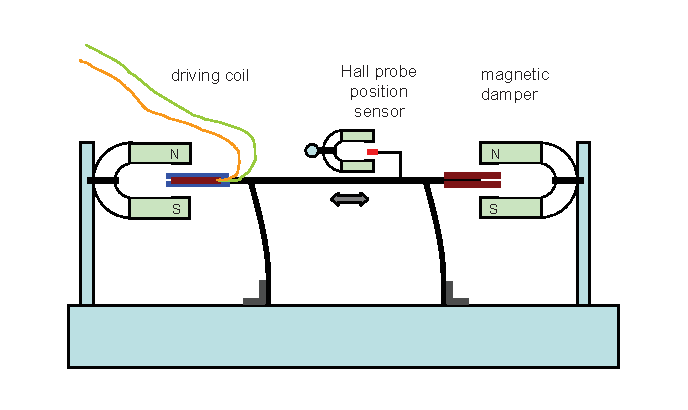
\includegraphics[width=4in]{ddhosetup.eps}
\caption{\label{ddhosetup}
Simplified diagram showing the principal components of the mechanical
oscillator studied in this experiment.  The bent vertical bars are the
flexible metal arms of a spring shown in the displaced position.  The
oscillations are from left to right in the figure.}
\end{figure}

The mechanical damped driven oscillator to be studied in this experiment
is similar to the one shown in Fig.~\ref{ddhosetup}.  The wires shown on
the left side of the figure connect to the coil mounted on the left end
of the oscillator beam.  When an ac current is sent through the coil, it
produces an alternating magnetic field in the vertical direction that
alternately repels and attracts the fixed permanent magnet mounted next to
it, to generate a driving force with a user-controlled amplitude and
frequency.  On the right end of the oscillator beam are mounted copper
strips which are inserted into the gap of a second fixed permanent magnet.
When the oscillator is in motion, eddy currents are produced in the copper
as a consequence of Faraday's Law, with a magnitude proportional to the
velocity of the oscillator.  The repulsion force between the permanent
magnetic and the magnetic dipole field arising from the eddy currents 
produces a drag force which opposes the direction of the motion of the
strips with a magnitude proportional to their velocity.  The ability to
move the permanent magnet in and out provides a user-controlled damping
force which acts in addition to the intrinsic damping of the oscillator due
to air drag and the inelasticity of the spring.

\subsection{position calibration}

The position of the oscillator is measured using a small electronic chip
containing a magnetic field sensor known as a Hall probe.  The Hall probe
works by passing an electric current through a ribbon-shaped conductor that
is oriented perpendicular to the local magnetic field whose intensity it
measures.  The Lorentz force on the current carriers in the metal strip
push them sideways as they move along the long axis of the ribbon, thus
inducing a potential difference between the left and right sides along the
entire length of the ribbon.  This potential difference, proportional to
the component of the magnetic field perpendicular to the plane of the
conductor, is known as the Hall voltage after physicist E.H.~Hall who
discovered this effect.  To function as a position sensor in this experiment,
the Hall probe is placed in the fringe field of a small permanent magnet
that is fixed to the laboratory bench.  It must be located in the fringe
field of the magnet, not in the center of the gap where the field of the
permanent magnetic is relatively constant, because it measures changes in
position by changes in the magnetic field.

The fringe field of the position-sensor magnet is a complicated non-linear
function of the Hall-probe sensor position, so the detailed functional
dependence of the Hall voltage on oscillator displacement $x$ must be
measured.  Once this is done, the function can be inverted to map any
measured Hall voltage to the corresponding displacement $x$.  To carry out
this calibration, remove the permanent magnet from the damping end of the
oscillator beam, and in its place mount a micrometer.  The micrometer is
a calibrated screw mounted on a heavy fixed stand that is marked off in
fine gradations of displacement.  Turn the micrometer to the middle of its
range and place it at the damping end of the oscillator beam so that the
screw axis is aligned with the oscillation direction and the micrometer tip
pushes against a solid flat surface on the end of the beam.  Move the base
of the micrometer mount to where the micrometer touches the oscillator in
its equilibrium position, and then do not move the mount again for the rest
of the calibration procedure.

Now back the micrometer out until contact
with the end of the beam is lost, then slowly advance it until it just
touches the beam.  Be careful not to jitter the oscillator during this step.
When completed, record the micrometer reading as the equilibrium value of
$x$, together with the Hall voltage $V$ that is displayed by the data
acquisition program.  Without moving the micrometer mount or the oscillator
support, advance the micrometer so that it pushes the beam toward the end
with the coil by less than 1~mm, and record the values of $x$ and $V$.

Repeat this procedure until you reach the end of the useful range of motion
of the oscillator.  Then back the micrometer out until the arm is free to
swing back through the equilibrium position all the way to the other end of
its normal range of swing.  Press the coil end of the arm gently until the
beam makes contact with the micrometer tip, and record the values of $x$
and $V$.  Once again advance the micrometer in small steps, recording $x$
and $V$ at each step, until you return to the equilibrium position.  You
may want to continue your measurements several steps past equilibrium and
repeat some of the measurements you made earlier just to check that nothing
moved during the calibration, and also to obtain an estimate of the 
measurement errors $\Delta V$ for a given $x$.

Enter these data into a
spreadsheet, and plot the recorded values with $x$ on the horizontal and
$V$ on the vertical axis.  A straight line generally will not provide a good
fit to these data.  Try a second or higher-order polynomial until a fit with
a good $\chi^2$ value is obtained.  The calibration function $x(V)$ you will
need for the remainder of the experiment is the inverse of the fit function
$V(x)$ you have just obtained.  If your $V(x)$ is linear or parabolic you
will be able to solve for the inverse function directly, otherwise you may
just want to rerun the fit with roles of $V$ and $x$ reversed.  Use the
same order polynomial in the new fit as you found produced a good $\chi^2$
value in the previous fit.  Record the coefficients of the best-fit
polynomial $x(V)$ for use in the following steps described below.

\subsection{impulse response measurement}

Remove the micrometer from the setup and start a data acquisition run
with no current going to the driving coil while the oscillator is visibly
motionless.  Even though the arm appears to be still, some variation should
still be present in the Hall voltage.  This comes about from vibrations in
the lab bench and the building that produce tiny oscillations of the system.
Notice that even though this external driving force is random, the response
of the system seems to have a single dominant frequency.  This is because of
the resonant character of the oscillator that picks out the Fourier component
of the random building vibrations at the resonant frequency and responds
primarily to it.  The amplitude fluctuates with time, as the response moves
in and out of 90$^{\circ}$ phase alignment with the random noise.  Familiarize
yourself with the level of this irreducible motion so that later on you will
not confuse it with the system response to a driving force you have introduced.

Gently tap the arm with the tip of a pen or pencil and watch the response.
A regular damped oscillation should appear on the Hall voltage.  It is normal
that the Hall voltage waveform should not look like a proper sine function.
This is because the Hall voltage is a nonlinear function of $x$.  Adjust
the sampling frequency of the data acquisition program until you are seeing
15-20 samples per oscillation period of the oscillator.  Adjust the total
acquisition time of a run until a single run contains the complete record of
a transient waveform from the instant it began until the motion has settled
down at the quiescent level determined in the previous step.  Record the
$V$ time series from the data acquisition program to a file, and then use a
spreadsheet to convert the $V$ time series into a $x$ time series using the
calibration function $x(V)$ obtained above.  Plot the function $x(t)$ and
verify that this does look like a decaying sine function.  If the calibration
procedure was successful, the $x$ waveform should look symmetric and
sinusoidal.  Experiment with different values for $\omega$ and $\Gamma$
that make Eq.~\ref{eq:dhosol} match your measured function $x(t)$.  You 
will need to adjust the initial values $x_0$ and $\delta_0$ to match the
initial amplitude and phase of the measured response before the two curves
will line up.

The coil mounted on the oscillator arm is capable of producing a more
reproducible impulse driving force than can be generated by hand.  Use the
data acquisition program to generate a large-amplitude current pulse in the
driving coil.  A 5~V pulse amplitude with a duration very short compared to
the free-running period of the oscillator, no more than 0.1~s, is required.
Ideally an impulse should have zero width, but you will probably have trouble
using a pulse much shorter than 0.05 seconds because the amplitude of the
motion will be so small that the signals will be very noisy. The main effect
of using a driving pulse with a finite width is to cause a small delay in the
response, which has little effect in the FFT analysis of the amplitude, but
is noticeable in the phase (see below).  Record 2 or 3 runs of the impulse
response using this driving pulse.  Then install the damping magnet around
the copper strips and repeat the measurement with two different values for
the damping coefficient $b$.

\subsection{sinusoidal response measurement}

Set the data acquisition program to generate a sinusoidal driving force near
the natural frequency of the oscillator that you observed in the previous
measurements.  Start out with a low value for the driving amplitude, and
increase it slowly until the magnitude of the oscillations reaches a high
but safe level of order 1~cm.  From the quiescent state, start the driving
and recording of the response waveform at the same time.  Be sure to record
data for a sufficiently long time to include both the transient and the
steady-state response to the driving force.  Because the transient and
steady-state terms in Eq.~\ref{eq:dhosol4} involve sine functions of 
different frequencies, regular beats are seen at the difference frequency
during the initial period while the transients are still present.  As soon
as the beats disappear and the oscillation amplitude becomes constant, you
know that the steady state has set in.

Record the amplitude of the response at the resonant frequency, then turn
down the driving frequency until the steady-state amplitude has decreased
by a factor 3.  Find the corresponding point above the resonance by increasing
$\omega_{_D}$ above $\omega_0$ until the amplitude once again is down by a
factor 3.  Now divide the interval between these two 1/3 points into 10
equal intervals and record sinusoidal response waveforms at each driving
frequency in between these limits.

\section{Data Analysis}

Your goal in the analysis of these data is to compare them with the
predictions of linear response theory, and to check for the presence and
significance of non-linear corrections.  The analysis tasks described
below involve many repetitions of the following two steps: convert a
measured Hall voltage time series $V(t)$ into a displacement times series
$x(t)$ and then fit the $x(t)$ data to a functional form by varying a set
of parameters to search for a minimum $\chi^2$.  Use the polynomial formula
obtained during the position calibration step to convert the values $V_i$
into displacements $x_i$.  You may have thousands of points per run to
convert, so using a spreadsheet or a program like Mathcad or MATLAB is
essential.  The following instructions are written with the spreadsheet
program Excel in view, but they can be easily carried out using the
equivalent functionality built into Mathcad or MATLAB as well.

To prepare for and carry out the fit, do the following.  Create two columns
to hold your measured data.  Add a label ``t (s)'' to the head of the first
column, and ``V (mV)'' to the head of the other.  Read or copy the data from
the data acquisition program into the two columns.  Create a third column
called ``$\Delta V$'' and enter into the top data cell the amplitude of
the Hall voltage fluctuations that you observe when the oscillator is
quiescent.  If you did not leave any free cells at the top of the spreadsheet
for future workspace, add free rows now.  In that upper workspace, use the
first column to write the names of the polynomial coefficients from your
fit to the $x(V)$ calibration data, and fill in the values next to them.
Down beside your data add columns 4 and 5 labeled ``x (cm)'' and
``$\Delta$ x''.  In the first data cell in the ``x'' column add the formula
involving the polynomial coefficients that converts the first $V$ value into
$x$.  Be sure to lock the coefficient references so that they do not slide
down when you copy the formula.  Then copy the top cell all the way down the
$x$ column.  In the $\Delta x$ column enter the same polynomial formula,
with the $\Delta V$ value substituted for the Hall voltage.  This will
serve as the error on the measured displacement $x$.  Using the same value
for $\Delta V$ and $\Delta x$ all rows in the table is OK.

The data are now ready to fit.  In the upper cell block add new labels for
the names of the parameters that are part of the formula that you want to
fit to the data.  In the cells next to the labels, enter initial values that
you guess based on what you expect their values to be.  These need not be
very close to the actual values; just about any reasonable guess will do.
Add new columns ``x fit'' and ``resid$^2$'' as columns 6 and 7 down in the main
data table.  Enter the fit formula into the top data cell in the ``x fit''
column, being careful to lock the cell addresses of the fit parameters,
and enter the formula taking the difference between the fit and measured $x$
values divided by $\Delta x$, all squared, into the ``resid$^2$'' column. 
Copy the top row to all of the rest of the rows in the table.  Up by the
fit parameters add the label ``$\chi^2$'' and enter there the formula that
sums all of the entries in the ``resid$^2$'' column.  Now use the Solver
to minimize the $\chi^2$ value by varying the free parameters in the fit.
If the fit is good, the best-fit $\chi^2$ value should be within a factor
2 of the number of samples in the time series you are analyzing.  If this
is not the case, investigate whether the problem lies with a poor estimate
of the errors or whether you may have made a mistake somewhere in the
formulas.

If the $\chi^2$ looks reasonable then the only thing remaining is to
extract the errors on the best-fit parameters from the fit.  When there
are only a dozen or so data points in a sample, the jackknife procedure is
useful for estimating fit parameters.  That method has the advantage that
it gives reliable answers even in the case where the errors are poorly
estimated.  However in a case like this with thousands of data points in the
fit, it is not a practical approach.  The alternate method to be used for
this experiment relies on having a good best-fit $\chi^2$ to begin with.
Assuming this is the case, proceed as follows to find the errors on the
best-fit parameter values.  Create a new row (or column) next to where
the best-fit parameter cells are located and label it ``errors'', then
next to ``errors'' add a new row (or column) that will be dedicated to
helping find the error on that parameter, and label it
``fixed {\em parameter}''.  For example, a fit with the 5 parameters 
$\omega_0$, $\Gamma$, $c_0$, $x_0$, and $\delta_0$ would have new rows
next to the error row labeled ``fixed $\omega_0$'', ``fixed $\Gamma$'',
``fixed $c_0$'', ``fixed $x_0$'', and ``fixed $\delta_0$''.  Provide an
initial guess for each of these parameter sets by copying the best-fit
values obtained earlier into each of the ``fixed {\em parameter}'' rows
(or columns).

Now, back in the original row (or column) where the best-fit
parameters are located, enter by hand a value for the first parameter that
is somewhat off from its best-fit value.  How much off it should
be is a matter of judgment, but you are trying to adjust it so that the
$\chi^2$ goes up by something in the range 1-2 or so.  It is not important
to be precise, just that it goes up by more than 0.1 and less than 10.
Use the Solver to repeat the fit with the same $\chi^2$ cell for the
minimization target, but this time excluding the parameter that you just
entered manually from the list of parameters to be varied in the fit.  All
of the other parameters except the one you have fixed should be left free in
the fit.  Because you have constrained the value of one of the parameters in
the fit, the $\chi^2$ will come out somewhat larger than the best-fit result,
but only by a little bit like 1-2, certainly less than 10 or you should move
the fixed parameter value closer to the best-fit value and try again.

Copy the values
of all of the fit parameters, and also the $\chi^2$ value from this fit into
the column ``fixed {\em parameter}'' for this parameter.  Be careful to use
{\em paste special = values} so that it copies the value of the $\chi^2$
from this fit and not the formula in the $\chi^2$ cell.  Proceed in this
way down the list of fit parameters, fixing each one slightly off its 
best-fit value and letting all of the other parameter vary freely in the fit.
When this is done you have everything you need to extract the errors on the
fit parameters.  The error for parameter $p$ is computed as
\begin{equation}
\Delta p = \frac{|p_1 - p_0|}{\sqrt{\chi^2_1-\chi^2_0}}
\label{eq:Deltap}
\end{equation}
where $p_0$ and $\chi^2_0$ are the values from the original best fit with
none of the parameters fixed, while $\chi^2_1$ is the value of $\chi^2$
returned from the fit with parameter $p$ fixed to value $p_1$.  Note that
there is only one value of $\chi^2_0$ for a given data set, but $n$ different
values $\chi^2_1$, one for each of the $n$ parameters in the fit.
In computing $\Delta p$ with Eq.~\ref{eq:Deltap}, do not forget that you
need to redo the all-free fit after all of the fixed-parameter fits have been
completed, so that the original values $p_0$, $\chi^2_0$ are set back
to their best-fit values on the spreadsheet.

\subsection{transient response}

Use the data analysis procedure outlined above to fit your transient
response data to a hypothesis of the form given in Eq.~\ref{eq:dhosol}.
All 4 parameters $x_0$, $\delta_0$, $\omega_0$, and $\Gamma$ should be
free parameters in the fit.  You should also introduce a fifth
parameter $x_{eq}$ to account for the non-zero value of the equilibrium
$x$-value around which the oscillations take place.
Make sure that the best-fit $\chi^2$ value
is reasonable.  Extract errors for the best-fit parameter $\Gamma$ and
the quantity $\omega$ based on best-fit parameters $\omega_0$ and $\Gamma$.
Repeat the analysis for each data set taken with under different damping
conditions.  Check the prediction from linear response theory that the
values $\omega_0$ from each of the fits should be the same within errors,
regardless of the value of the damping constant $\Gamma$.  Check that
the data sets with larger damping force have larger values of $\Gamma$,
and that these variations are well outside the error bars.

\subsection{sinusoidal driver response}

Use the data analysis procedure outlined above to fit your data that
were taken in the presence of a sinusoidal driving force to the general
form given in Eq.~\ref{eq:dhosol4}, interpreting the measured value as the
real part of the complex function $x$ in Eq.~\ref{eq:dhosol4}, which can
be written as follows.
\begin{equation}
x(t) = x_{eq} + x_0 e^{-\Gamma t} \sin(\omega t + \delta_0) 
              + A \sin(\omega_{_D} t + \phi)
\label{eq:dhosol4R}
\end{equation}
There should be a total of 8 free parameters in the fit: the original
set $x_{eq}$, $x_0$, $\delta_0$, $\omega_0$, and $\Gamma$ used in the
transient response analysis, and the 3 new free parameters describing
the steady-state response which are $\omega_{_D}$, $|A|$, and $\phi$.

To interpret the value of $\phi$, you also need to measure the phase
of the driving force. When you collected the data for the steady-state
response, you should also have recorded the driving waveform that went
with it. The driving waveform can be fit to a similar formula to
Eq.~\ref{eq:dhosol4R} with its own values for $x_{eq}$, $|A|$, and $\phi$.
This is the driving term so there is no transient part, which means
you can set $x_0=0$ in this fit and leave out fit parameters $\Gamma$,
$\omega_t$, and $\delta_0$.  The object of this fit is to extract the 
amplitude and phase of the driving force, which you can call $|A_{_D}|$
and $\phi_{_D}$ to distinguish them from the $|A|$ and $\phi$ that were
obtained from the fit to the oscillator response data. In the end,
what you will want to get from these fits are the amplitude ratio
$|A/A_{_D}|$, and the difference $\phi - \phi_{_D}$ which is called
the ``phase shift.''

Repeat the above analysis for all 10 data sets which you took at different
frequencies $\omega_{_D}$ around the resonance peak.  Check that all of
the values of $\omega_{_D}$ returned from the fits are consistent with the
frequency settings selected for the driving force.  Plot the values of
the amplitude ratio and the phase shift as functions of driving force
$\omega_{_D}$.  The errors from the fit procedure described above should be
included on the plot as vertical error bars.  On the same plots, draw curves
for the predicted functional form of $|A|$ and $\phi$ given in
Eq.~\ref{eq:AofwMP}, using the values of $\omega_0$ and $\Gamma$
that you obtained from the analysis of the transient response under
the same damping conditions as were used
for the measurements with the sinusoidal driver.  These curves are 
predictions for the behavior of the amplitude ratio and the phase shift
without any free parameters, so there is no fit to be done at this point.
Compute the $\chi^2$ for these data against the functions predicted by
linear response theory.

\subsection{non-linear corrections}

In the introduction it was pointed out that linear response theory cannot
describe certain aspects of a physical damped oscillator, such as damping
caused by ordinary surface friction.  The solution to the equation of 
motion that includes a non-linear term due to surface friction was given
in closed form in Eq.~\ref{eq:dhosol2}.  This piece-wise expression can
be approximated as a single analytic function in the case where the constant
$c_0$ is small compared to the initial amplitude $x_0$, which is the case
in this experimental setup.  The approximate solution in the case where
$F=0$ is
\begin{equation}
x(t) = \left\{\begin{array}{lll}
\left(x_0-\frac{2c_0\omega}{\pi}t\right)\,
e^{-\Gamma t}\sin(\omega t + \delta_0) &:& t<\frac{\pi x_0}{2c_0\omega} \\
0 &:& ow
\end{array} \right.
\label{eq:dhosol2a}
\end{equation}
Fit your transient response data sets to the form Eq.~\ref{eq:dhosol2a}
with new free parameter $c_0$ in addition to the familiar parameters
$x_0$, $\delta_0$, $\omega_0$, and $\Gamma$.  Extract errors for these
fit parameters, and check whether including the non-linear term significantly
improved the fit.  One way to check this is to see if the $\chi^2$ value
decreased by more than 1.  Other way is to look and see if the value of
the $c_0$ is consistent with 0 within its error.  Comment on what physical
sources of damping might contribute through the parameter $\Gamma$ and
which ones would be expected to show up in $c_0$.

%\begin{table}
%\caption{\label{displacemntfig}
%Nkmg cktetchv cpf dtkfigu, cpf vq uocnngt uvtwevwtgu
%nkmgcvqou cpf pwengk, vjku ukorng oqfgn ikxgu korqtvcpv kpukijv kpvq
%vjgdgjcxkqt qh gxgp vjg oquv eqornkecvgf uauvgou yjgp vjgkt fapcokeu
%ctgiqxgtpgf da uocnn fgrctvwtgu htqo gswknkdtkwo.}
%\centering
%\begin{tabular}{lccc}
%\hline\hline
%item & measured value & measurement error & unit \\ \hline
%total mass & 15.67 & 0.02 & kg \\
%length eyes-tailfin & 14.6 & 0.05 & cm \\
%height belly-dorsal & 3.98 & 0.05 & cm \\
%flash response time & 1.23 & 0.15 & s \\
%total turn time & 1.08 & 0.05 & s \\
%turn radius & 0.72 & 0.15 & cm \\
%maximum turn velocity & 22.1 & 0.5 & m/s \\
%\hline\hline
%\end{tabular}
%\end{table}

\begin{acknowledgments}
This document was prepared by Prof. Richard Jones, based on an earlier
write-up by Prof. Ed Eyler (2005).
\end{acknowledgments}

%% Create the reference section using BibTeX:
%\bibliography{revtex4}

%\begin{thebibliography}{9}
%
%\bibitem{Tznpo71}
%Lfjui S. Tznpo,
%\emph{Nfdibojdt},
%Beejtpo-Xftmfz, Sfbejoh NB,
%3se fe. (1971) pp. 214-215.
%
%\bibitem{Lmfqqofs73}
%E. Lmfqqofs boe S.K. Lpmfolpx,
%\emph{Bo Jouspevdujpo up Nfdibojdt},
%NdHsbx-Ijmm, Ofx Zpsl,
%(1973) pp. 257-257.
%
%\bibitem{Nbsjpo95}
%K.C. Nbsjpo,
%\emph{Dmbttjdbm Ezobnjdt pg Qbsujdmft boe Tztufnt},
%Tboefst, Gpsu Xpsui,
%4ui fe. (1995) p. 455.
%
%\bibitem{Ifjtlbofo67}
%X.B. Ifjtlbofo, boe I. Npsjua,
%\emph{Qiztjdbm Hfpeftz},
%X.I. Gsffnbo, Tbo Gsbodjtdp
%(1967).
%
%\end{thebibliography}

\end{document}
%%
%% ****** End of file template.aps ******
%%
